\chapter{Conceptos teóricos}

En este capítulo se describen (brevemente) todos los conceptos necesarios para entender el trabajo. No se trata de copiar el contenido de los libros de texto, si no de hacer un resumen de los conceptos necesarios para facilitar la lectura del documento al lector. Se entiende que el lector de un TFG tiene que tener unos conocimientos mínimos sobre el tema.

\section{¿Qué es la domótica?}

mimi

\section{Marco histórico}

mimi

\section{¿Qué es KNX?}

knx, protocolos, teoria clase...)

\section{Lista de materiales}

A continuación, se detalla una lista con los múltiples dispositivos y módulos domóticos que han sido utilizados para desarrollar la solución final diseñada y la funcionalidad que les ha sido otorgada. En esta lista únicamente aparecerán los elementos incluidos en el cuadro eléctrico de domótica y los mecanismos domóticos de la instalación, quedando excluidos, por tanto, los efectores y actuadores puramente eléctricos así como su cuadro, por no encontrarse dentro de las competencias de diseño del sistema.

\subsection{Actuadores} Estos elementos se encargan de ejecutar las acciones solicitadas desde el controlador sobre los diferentes elementos domóticos de la vivienda a los que se encuentra conectado. Existen diversas clases de actuadores que se clasifican en función de la aplicación que vayan a desarrollar. En este proyecto se utilizarán los siguientes:

\begin{itemize}
\item \textbf{Dimmers:} 
	\begin{itemize}
	\item\underline{Descripción:} actuador regulador KNX de 4 elementos.
	\item \underline{Características:} este tipo de actuador permite el control de la regulación del elemento que se encuentra conectado a su salida mediante el uso de dispositivos TRIAC y DIAC. Cuenta con modo de accionamiento manual para modo de prueba, además de protección contra marcha en vacío, cortocircuito y sobretemperatura. 
	\item \underline{Funcionalidad:} la aplicación que ejecutan es la de regulación de la intensidad de la iluminación de algunas de las lámparas de la vivienda.\\ [0,15 cm]
		\begin{figure}[h]
		\centering
		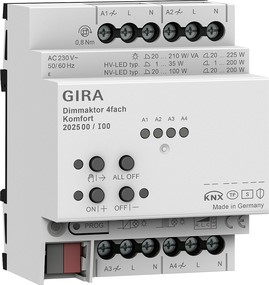
\includegraphics[width=0.35\textwidth]{figures/actuador_dimmer.jpg}   
		\caption{Actuador tipo dimmer}
		\label{fig:actuador_dimmer}
		\end{figure}
	\end{itemize} 


\item \textbf{Binario + persiana:} 
	\begin{itemize}
	\item\underline{Descripción:} actuador de conmutación de 24 elementos / control 12 persianas.
	\item \underline{Características:} este módulo combina la funcionalidad de dos tipos de actuadores diferentes, y permite el control tanto de elementos ON/OFF como de persianas, atendiendo a la funcionalidad con la que se programen sus salidas. Cuenta con modo de accionamiento manual para modo de prueba.
	\item \underline{Funcionalidad:} algunas de sus salidas serán utilizadas para el control de apertura de una ventana y el despliegue de una pantalla de proyección. El resto servirán para el control binario del resto de luces de la casa y de algunas de las tomas de corriente que se han decidido “domotizar”. Otras funcionalidades puntuales de tipo binario que tienen sus salidas son las de accionamiento del timbre, de la sirena de alarma, el control de la cerradura de la vivienda, la velocidad del recuperador, el encendido de la caldera y las electroválvulas de agua y gas.
	\begin{figure}[h]
	\centering
	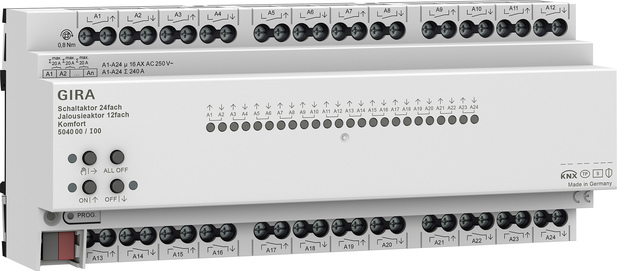
\includegraphics[width=0.55\textwidth]{figures/actuador_binario.png}   
	\caption{Actuador tipo binario/persiana}
	\label{fig:actuador_binario}
	\end{figure}
	\end{itemize} 

\item \textbf{Rejilla + zonificación:} 
	\begin{itemize}
	\item\underline{Descripción:} actuador de control sobre 8 rejillas + 2 unidades de aire acondicionado.
	\item \underline{Características:} esta clase de actuador combina la capacidad de control de la apertura de una rejilla con la de gestión de diferentes temperaturas mediante módulos lógicos. . Cuenta con modo de accionamiento manual para modo de prueba, además de indicadores visuales de movimiento de rejillas mediante LEDs.
	\item \underline{Funcionalidad:} gracias a sus características, nos permite conectarlo con los termostatos distribuidos por la casa y hacer un control por zonas de la distribución del sistema de aerotermia de los fancoils, activando y adecuando la velocidad de sus ventiladores en función de la demanda.
	\begin{figure}[h]
	\centering
	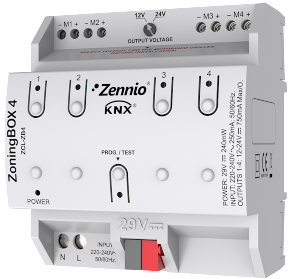
\includegraphics[width=0.35\textwidth]{figures/actuador_rejilla.png}   
	\caption{Actuador tipo zonificación}
	\label{fig:actuador_rejilla}
	\end{figure}
	\end{itemize} 

\item \textbf{Accionamiento térmico:} 
	\begin{itemize}
	\item\underline{Descripción:} actuador de calefacción de 6 elementos.
	\item \underline{Características:} permite la actuación de accionamientos térmicos integrado con un regulador de temperatura ambiente. Incluye la opción del conexionado en cascada de los actuadores.
	\item \underline{Funcionalidad:} las salidas de este módulo irán conectadas a las válvulas de regulación de los entramados del suelo radiante para regular su apertura, así como a la caldera de la vivienda, indicando los momentos en los que esta debe ser activada en función de la demanda de temperatura gestionada por los termostatos. \\ [0,15 cm]
	\begin{figure}[h]
	\centering
	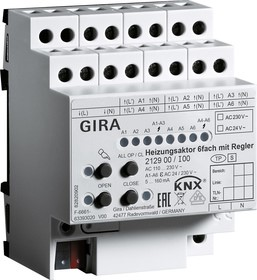
\includegraphics[width=0.35\textwidth]{figures/actuador_termico.jpg}   
	\caption{Actuador tipo térmico}
	\label{fig:actuador_termico}
	\end{figure}
	\end{itemize} 
\end{itemize} 

\subsection{Sensores}

\begin{itemize}
\item \textbf{CO\textsubscript{2}:} 
	\begin{itemize}
	\item\underline{Descripción:} sensor CO\textsubscript{2} con regulador de humedad y temperatura KNX.
	\item \underline{Características:} supervisión del valor de partículas de \textsubscript{2} y de humedad en el ambiente. Alarma de punto de rocío para prevenir la formación de moho en sistemas de refrigeración. Posee dos entradas binarias para la conexión de contactos sin tensión. El sensor de \textsubscript{2} permite ajustar cuatro niveles límites diferentes.
	\item \underline{Funcionalidad:} la funcionalidad con la que ha sido programado es la de, mediante la actuación de tres niveles de partículas de \textsubscript{2}, activar los tres niveles de velocidad del ventilador del recuperador en consecuencia.
	\begin{figure}[h]
	\centering
	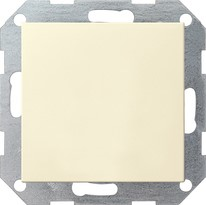
\includegraphics[width=0.30\textwidth]{figures/sensor_co2.jpg}   
	\caption{Sensor de CO\textsubscript{2}}
	\label{fig:sensor_co2}
	\end{figure}
	\end{itemize} 


\item \textbf{Movimiento:} 
	\begin{itemize}
	\item\underline{Descripción:} detector de movimiento de superficie de 2,2 m.
	\item \underline{Características:} configurable para la detección de movimiento o para la monitorización del con capacidad de cuantificar la luminosidad de la estancia para realizar un apagado de la iluminación al superar un umbral configurable. Permite la configuración de un bloque de función para realizar las siguientes funciones: conmutación, función para escaleras, transmisor de valores de regulación, mecanismo auxiliar para escenarios, transmisor de valores de temperatura, transmisor de valores de luminosidad, conmutación de modo de funcionamiento, conmutación con posición forzada.
	\item \underline{Funcionalidad:} serán utilizados para detectar la entrada de personas en determinadas zonas de la vivienda, y en función del modo en que se encuentre el sistema, hará las veces de ON/OFF de las luces de esas zonas o bien hará saltar el sistema de alarma ante intrusiones.
	\begin{figure}[h]
	\centering
	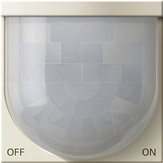
\includegraphics[width=0.25\textwidth]{figures/sensor_movimiento.png}   
	\caption{Sensor de movimiento}
	\label{fig:sensor_movimiento}
	\end{figure}
	\end{itemize} 

\item \textbf{Presencia:} 
	\begin{itemize}
	\item\underline{Descripción:} detector presencia multifunción.
	\item \underline{Características:} posee varios modos de funcionamiento, a saber: detector de presencia, observador de techo o detector de movimiento. La monitorización del entorno se realiza mediante el uso de tres sensores PIR y uno de luminosidad, con lo que se permite utilizar los parámetros de detección de las tres zonas y de luminosidad para hacer un control en intensidad de la iluminación zonal en sintonía con la posibilidad de utilizar las cinco funciones lógicas que permite usar. La funcionalidad de este dispositivo es similar a la del detector de movimiento, pero con los siguientes añadidos: transmisión de valores de regulación, nivel crepuscular ajustable, aplicación de retardos, función de bloqueo y la posibilidad de configuración de límites de luminosidad.
	\item \underline{Funcionalidad:} gracias a su diseño discreto, se instala en el techo del salón con la funcionalidad de controlar la iluminación de la estancia en función de principalmente dos parámetros externos: la presencia de personas y la iluminación exterior, aplicándole un valor de sensibilidad determinado para realizar el ON a partir de la detección de cierta cantidad de luxes.
	\begin{figure}[h]
	\centering
	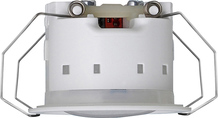
\includegraphics[width=0.35\textwidth]{figures/sensor_presencia.png}   
	\caption{Sensor de presencia}
	\label{fig:sensor_presencia}
	\end{figure}
	\end{itemize}

\item \textbf{Inundación:} 
	\begin{itemize}
	\item\underline{Descripción:} sensor de inundación.
	\item \underline{Características:} es capaz de detectar la presencia de agua en un ambiente.
	\item \underline{Funcionalidad:} será necesario la implementación de un módulo de entradas para poder comunicar los sensores con la instalación KNX de la vivienda.
	\begin{figure}[h]
	\centering
	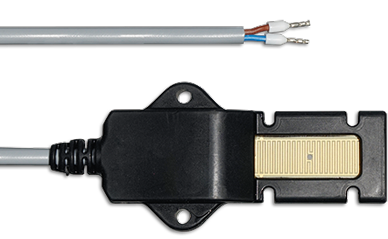
\includegraphics[width=0.35\textwidth]{figures/sensor_inundacion.png}   
	\caption{Sensor de inundación}
	\label{fig:sensor_inundacion}
	\end{figure}
	\end{itemize} 

\item \textbf{Apertura:} 
	\begin{itemize}
	\item\underline{Descripción:} contacto magnético.
	\item \underline{Características:} este sensor consta de dos partes: la primera irá fijada en el marco de la ventana y la segunda, en la propia ventana. Al cerrar la ventana, se cerrará el circuito eléctrico, transmitiendo así un valor por el bus opuesto al que envía al encontrarse abierto.
	\item \underline{Funcionalidad:} su misión será la de ofrecer al sistema información acerca de si las ventanas de la casa se encuentran abiertas o cerradas.
	\begin{figure}[h]
	\centering
	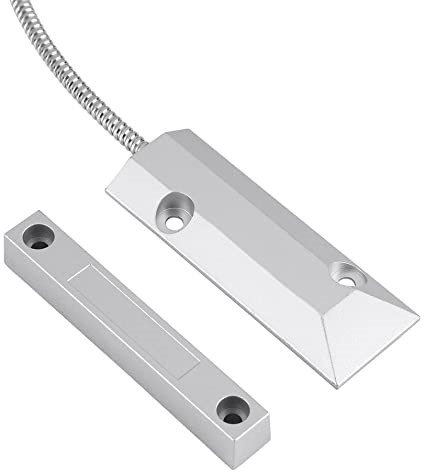
\includegraphics[width=0.35\textwidth]{figures/sensor_apertura.png}   
	\caption{Sensor de apertura}
	\label{fig:sensor_apertura}
	\end{figure}
	\end{itemize} 

\item \textbf{Humo:} 
	\begin{itemize}
	\item\underline{Descripción:} combinación de detector de humos y detector térmico.
	\item \underline{Características:} sensor termovelocimétrico alimentado por pilas. Dos señales acústicas de alarma distintas para cada uno tipos de detección con posibilidad de atenuarse durante la fase de pruebas.
	\item \underline{Funcionalidad:} su objetivo es el de detectar de situaciones anómalas y potencialmente peligrosas relacionadas con los incendios y dar aviso de ello a los usuarios que se encuentren en la vivienda. Para poder ser integrados en la instalación KNX, será necesario la implementación de un módulo extra, que será el encargado de comunicar el detector de humos con el sistema de control de la vivienda.
	\begin{figure}[h]
	\centering
	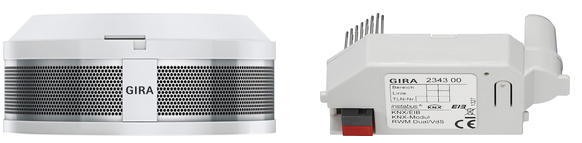
\includegraphics[width=0.75\textwidth]{figures/sensor_humo.png}   
	\caption{Sensor de humo y módulo KNX}
	\label{fig:sensor_humo}
	\end{figure}
	\end{itemize} 
\end{itemize} 

\subsection{Lectores de consumo}

\begin{itemize}
\item \textbf{Electricidad:} 
	\begin{itemize}
	\item\underline{Descripción:} medidor de energía eléctrica para sistemas monofásicos o trifásicos.
	\item \underline{Características:} permite el monitorizar la energía consumida/producida, el coste y las emisiones de \textsubscript{2} asociadas al consumo, la potencia activa y reactiva, el factor de potencia y otra información relacionada con el uso de la energía en la vivienda.
	\item \underline{Funcionalidad:} se monitorizarán la tensión y corriente de fase instantáneos, la potencia activa consumida instantánea y la energía consumida acumulada total y en un periodo de tiempo definido por el usuario, incluyendo la tarifa y sus emisiones de carbono en esos periplos. Se realizarán dichas medidas acoplando un transformador de corriente a cada una de las líneas. 
	\begin{figure}[h]
	\centering
	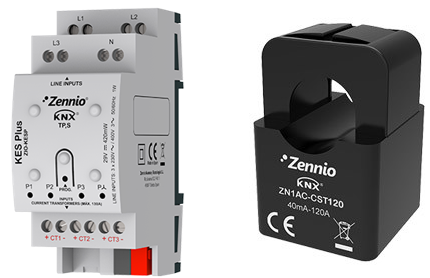
\includegraphics[width=0.55\textwidth]{figures/contador_electricidad.png}   
	\caption{Contador consumo eléctrico y acoplador de línea }
	\label{fig:contador_electricidad}
	\end{figure}
	\end{itemize} 

\item \textbf{Agua y gas:} 
	\begin{itemize}
	\item\underline{Descripción:} interfaz KNX de monitorización de consumo de 4 elementos.
	\item \underline{Características:} permite monitorizar en el bus KNX el consumo eléctrico (energía y potencia), agua y gas mediante el conteo de pulsos SO (salida impulso optoacoplador). Estas medidas pueden visualizarse en consumo instantáneo o acumulado.
	\item \underline{Funcionalidad:} estos módulos serán utilizados para hacer un conteo del consumo acumulado total y desdeuna fecha determinada por el usuario del agua y el gas gastados en la vivienda. Tambien se utilizará su funcionalidad de calculo de tarifas, para que el cliente pueda consultar el gasto en cualquier periplo. Irá conectado directamente a los instrumentos de medida de la vivienda.
	\begin{figure}[h]
	\centering
	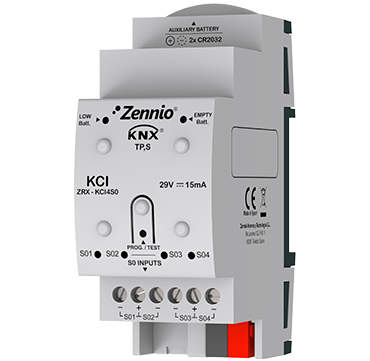
\includegraphics[width=0.35\textwidth]{figures/contador_agua.png}   
	\caption{Contador de consumo de agua y gas}
	\label{fig:contador_agua}
	\end{figure}
	\end{itemize} 
\end{itemize} 

\subsection{Interfaces del usuario}

\begin{itemize}
\item \textbf{Pulsadores domóticos:} 
	\begin{itemize}
	\item\underline{Descripción:} mecanismo acoplador de bus.
	\item \underline{Características:} de la variedad de características que pueden presentar este tipo de elementos, se han escogido los acopladores de bus con pulsación sobre dos elementos con mando de un punto, es decir, pulsadores de dos teclas con posibilidad de pulsarse únicamente en una dirección. 
	\item \underline{Funcionalidad:} control de las lámparas, tanto las binarias como las dimmeables, los enchufes, activación de las velocidades del recuperador, subir y bajar la pantalla del proyector, abrir y cerrar la ventana y activación del timbre.
	\begin{figure}[h]
	\centering
	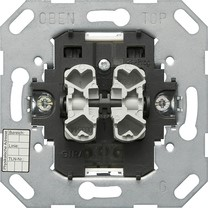
\includegraphics[width=0.30\textwidth]{figures/pulsador.jpg}   
	\caption{Pulsadores domóticos}
	\label{fig:pulsador}
	\end{figure}
	\end{itemize} 

\item \textbf{Termostatos:} 
	\begin{itemize}
	\item\underline{Descripción:} panel táctil capacitivo con display.
	\item \underline{Características:} posee 4 botones con multidisplay de 4 indicadores personalizables. Incluye funcionalidad de termostato, detector de movimiento y 2 puertos de entradas de tipo binario o lectura desde una sonda de temperatura.
	\item \underline{Funcionalidad:} se utilizará su función de termostato para gestionar el sistema de climatización. Desde estos dispositivos se efectuarán las llamadas de demanda tanto al sistema de suelo radiante como a los fancoils, en función de las temperaturas sensadas en cada habitación mediante el uso de una de sus entradas como sonda de temperatura. Uno de los termostatos llevará en su segunda canal de entrada una sonda térmica utilizada para conocer la temperatura exterior a la vivienda. Además, sus botones serán utilizados para las siguientes funciones:
		\begin{itemize}
		\item Los botones en el cuadrante inferior serán utilizados para subir y bajar la temperatura de consigna de la zona en la que se encuentra el termostato.
		\item El botón en el cuadrante superior derecho tendrá la funcionalidad de variar el flujo de aire cedido por los equipos de aire acondicionado. Al ser un único botón, la secuencia que efectuará será cíclica con el siguiente patrón: +, ++, +++, A, +. ++, +++, A, … Siendo A la ejecución del modo automático, que seleccionará la velocidad de los ventiladores en función de la demanda y la ponderación otorgada a cada zona o habitación.
		\item El botón en el cuadrante superior izquierdo servirá para cerrar la rejilla de esa habitación, evitando así el paso del aire de los fancoils.
		\end{itemize} 
	\begin{figure}[h]
	\centering
	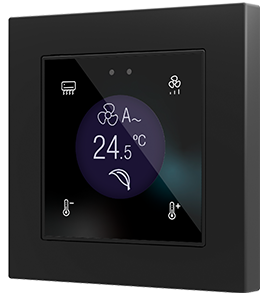
\includegraphics[width=0.37\textwidth]{figures/termostato.png}   
	\caption{Termostato}
	\label{fig:termostato}
	\end{figure}
	\end{itemize} 

\item \textbf{G1:} 
	\begin{itemize}
	\item\underline{Descripción:} es un dispositivo multifunción que permite visualizar y controlar numerosas funciones del edificio relacionadas con el control de los módulos instalados en ellos.
	\item \underline{Características:} posee una infinidad de funcionalidades, por lo que se mencionan únicamente las que poseen un enfoque más focalizado hacia las buscadas en este proyecto: una pantalla táctil con altavoz y micrófono integrados, capacidad de reconocimiento facial y reproducción de vídeo. Es posible personalizar su interfaz de usuario con la posibilidad de utilizar más de 320 iconos de función organizadas por carpetas con un manejo muy intuitivo. 
	\item \underline{Funcionalidad:} será utilizado como monitor y como puesto de control principal de la vivienda, representando la programación volcada sobre el X1. Esta pantalla hará las veces de display para mostrar las cadenas de texto o los datos que puedan resultar de interés para el usuario, como pudieran ser mensajes de alarma, de consumo, de avería o error... 
	\begin{figure}[h]
	\centering
	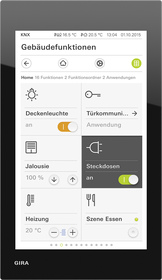
\includegraphics[width=0.25\textwidth]{figures/g1.png}   
	\caption{G1}
	\label{fig:g1}
	\end{figure}
	\end{itemize} 
\end{itemize} 

\subsection{Módulos de entradas}

\begin{itemize}
\item \textbf{Para sensores de apertura:} 
	\begin{itemize}
	\item\underline{Descripción:} entrada binaria KNX de 6 elementos.
	\item \underline{Características:} este módulo posee 6 entradas binarias que transforman sus valores en telegramas KNX. Permite ejecutar dos acciones diferentes por cada flanco, tanto de subida como de bajada, de cada una de las salidas.
	\item \underline{Funcionalidad:} en este proyecto, este mecanismo tendrá como entradas una serie de contactores magnéticos, cuya tarea es la de sensar el estado de las ventanas (abierto o cerrado), para que, en caso de pasar una cantidad de tiempo determinada en estado abierto, desconecte el sistema de climatización para esa estancia.
	\begin{figure}[h]
	\centering
	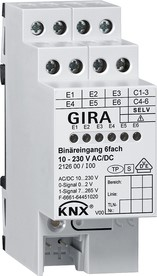
\includegraphics[width=0.2\textwidth]{figures/entradas_apertura.jpg}   
	\caption{Módulo 6 entradas para sensores de apertura}
	\label{fig:entradas_apertura}
	\end{figure}
	\end{itemize} 
\end{itemize} 

\subsection{Pasarelas}

\begin{itemize}
\item \textbf{Para sistema de aerotermia:} 
	\begin{itemize}
	\item\underline{Descripción:} pasarela Daikin – KNX.
	\item \underline{Características:} permite la comunicación bidireccional entre los sistemas Daikin VRV y las instalaciones KNX. 
	\item \underline{Funcionalidad:} su principal misión será la de servir de puente de comunicación entre el sistema propio de los sistemas de fancoil de la vivienda y el sistema domótico KNX, permitiendo así su control a través del bus mediante el envío de telegramas y su decodificación.
	\begin{figure}[h]
	\centering
	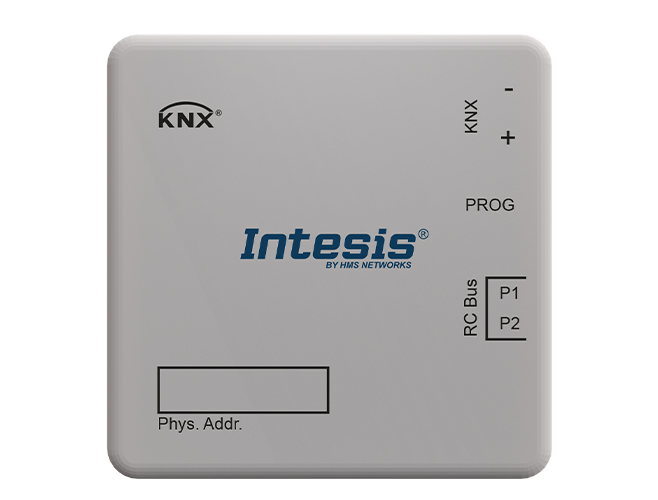
\includegraphics[width=0.47\textwidth]{figures/pasarela.png}   
	\caption{Pasarela para sistema de aerotermia}
	\label{fig:pasarela}
	\end{figure}
	\end{itemize} 
\end{itemize} 

\subsection{Servidores}

\begin{itemize}
\item \textbf{X1:} 
	\begin{itemize}
	\item\underline{Descripción:} servidor de visualización para terminales móviles.
	\item \underline{Características:}  este mecanismo permite la visualización de una interfaz personalizada en tu móvil o tablet  a través de internet, así como el control de hasta 250 funciones mediante el uso de comandos de voz o bien mediante la aplicación. Capacidad de uso de hasta 250 temporizadores, 36 bloques lógicos diferentes y 1450 datapoints.
	\item \underline{Funcionalidad:} contendrá los módulos lógicos programados para desarrollar las funcionalidades especiales del resto de módulos y el software sobre el que se programa la interfaz de visualización tanto del G1 como de la aplicación móvil. También permitirá la conexión remota a través de la aplicación móvil al alojar un servidor propio a través de la conexión Wi-Fi de la vivienda.
	\begin{figure}[h]
	\centering
	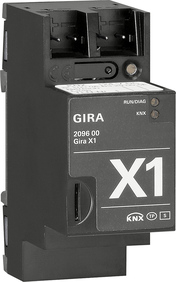
\includegraphics[width=0.23\textwidth]{figures/x1.png}   
	\caption{X1}
	\label{fig:x1}
	\end{figure}
	\end{itemize} 
\end{itemize} 

\subsection{Fuentes de alimentación}

Esta función será desarrollada por un módulo único compartido por ambos cuadros domóticos de la vivienda. Su cometido es el de transformar la corriente alterna proveniente de la acometida pública que llega a las casas con una tensión de 230V entre fase y neutro, en corriente continua de 29V, que es el potencial de bus necesario para alimentar los dispositivos. Este dispositivo no cuenta con ningún tipo de distribuidor de intensidad, por lo que la corriente nominal será repartida de manera discrecional en las salidas, hasta un máximo de 640 mA. Para prevenir posibles comportamientos anómalos de la red eléctrica, este dispositivo cuenta con una bobina de choque integrada en su interior, un componente electrónico de muy alta reactancia que hará las veces de filtro de las corrientes alternas, eludiendo futuras fallas o roturas de los mecanismos domóticos..
\begin{figure}[h]
\centering
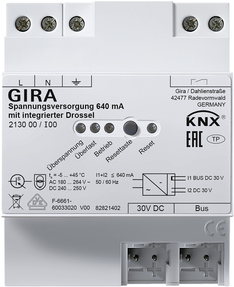
\includegraphics[width=0.3\textwidth]{figures/fuente_alimentacion.png}   
\caption{Fuente de alimentación}
\label{fig:fuente_alimentacion}
\end{figure}
